% Indicate the main file. Must go at the beginning of the file.
% !TEX root = ../main.tex

%%%%%%%%%%%%%%%%%%%%%%%%%%%%%%%%%%%%%%%%%%%%%%%%%%%%%%%%%%%%%%%%%%%%%%%%%%%%%%%%
% 03_methods
%%%%%%%%%%%%%%%%%%%%%%%%%%%%%%%%%%%%%%%%%%%%%%%%%%%%%%%%%%%%%%%%%%%%%%%%%%%%%%%%

\section{Methods}
\label{methods}

    \subsection{Dataset}

    As part of the Wildlife@Campus project, a labeled dataset was created to train a deep learning algorithm.
    The information about the dataset is derived from the dataset itself and a progress report available on GitHub \autocite{ratnaweeraWildlifeCampusProgressReports2021}.
    This dataset is divided into seven sessions -- indicating the source of the images -- the sessions and their origin are listed in \autoref{tab:session_info}.
    The dataset provides two kinds of labels: the original annotations from each session, and a standardized version created when the sessions were integrated into the dataset.
    For this project, only the standardized labels where used.
    Images group into sequences, with each sequence representing a single animal sighting.
    The sequences where created by the Wildlife@Campus team, utilizing the EXIF information of the images to group them based on the time and date of the capture.
    Sequence lengths vary and can span anywhere from 1 up to 915 images.
    
    To get an overview of the available sequences per label, refere to \autoref{fig:sequenceperlabel}.
    The category \texttt{other} represents sequences containing more than one species, this is a result of the process creating the sequences.
    Furthermore, the category \texttt{NaN} represents sequences not labeled -- both where excluded from the from the dataset.
    The category \texttt{glis\_glis} is represented in only four sequences, which is simply not enough to actually train a model to detect it.
    For this reason, it was excluded from the dataset as well.
    This leaves four categories for the classification task: \texttt{apodemus\_sp}, \texttt{cricetidae}, \texttt{soricidae}, and \texttt{mustela\_erminea}.

    %==== table: overview_dataset ====%
    \begin{table}[H]
\caption{Information about the origin of the different sessions in the dataset.}
\label{tab:session_info}
\begin{tabular}{c p{12cm}}
\toprule
Session & Description \\
\midrule
1 & Data from 'the wild', collected durch Wiesel\&Co 2019 \\
2 & Data from 'the wild', collected during WILMA (SummerSchool) 2020 \\
3 & Data from 'the wild', collected by Vogelwarte 2020 \\
4 & Data from 'the wild', collected by WILMA (Bachelorthesis) 2020 \\
5 & Data from 'the wild', collected by WILMA (Roland) 2020 (Contains images and videos of stoats (Mustela erminea)) \\
6 & Data from an enclosure, collected by Nils (Contains only images of stoats (Mustela erminea)) \\
7 & Data gathered from Nathalie Straub in her Bachelor Thesis \\
\bottomrule
\end{tabular}
\end{table}

    %=================================%

    \begin{figure}[ht]
    \centering
    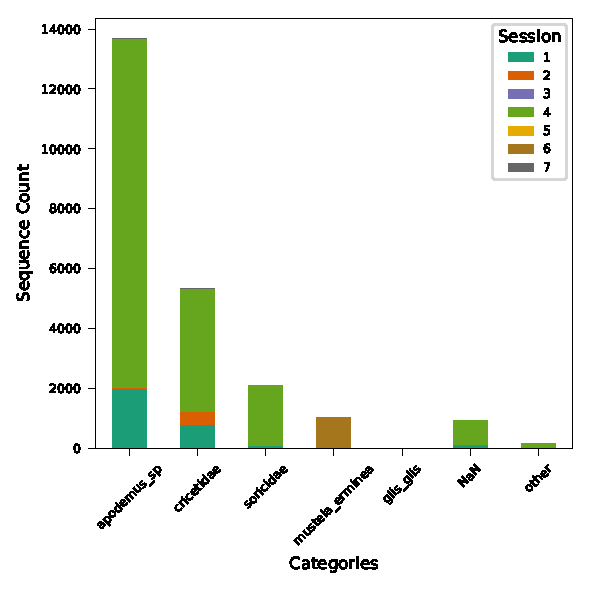
\includegraphics{figures/label2_session.pdf}
    \caption{Available sequences per label colored by session.}
    \label{fig:sequenceperlabel}
    \end{figure}

    \subsection{Data Processing}

    The processing of the images is divided into two main steps: 
    In a first step a detector is applied to identify the regions of interest (ROI) for the images, and to select which images are actually used for training.
    In a second step, the ROIs are processed to be feed into the model.

        \subsubsection{Detection and Selection}
        
        In this project, the Megadetector (MD) \autocite{morrisEfficientPipelineCamera2025} is used to identify regions of interest (ROI) on all the images.
        The MD outputs a list of bounding boxe (BBox) for detected objects labeled \textit{animal}, \textit{human} or \textit{vehicle} with a corresponding confidence value.
        For each image only the BBox with the highest confidence score -- above a threshold of 0.5 -- for the label \textit{animal} is considered.
        The percentage of images discarded dew to this process is  shown per sequence in \autoref{fig:lost_images}.
        An example of how this detections look like is shown in \autoref{fig:detection_example}.

        \begin{figure}[ht]
        \centering
        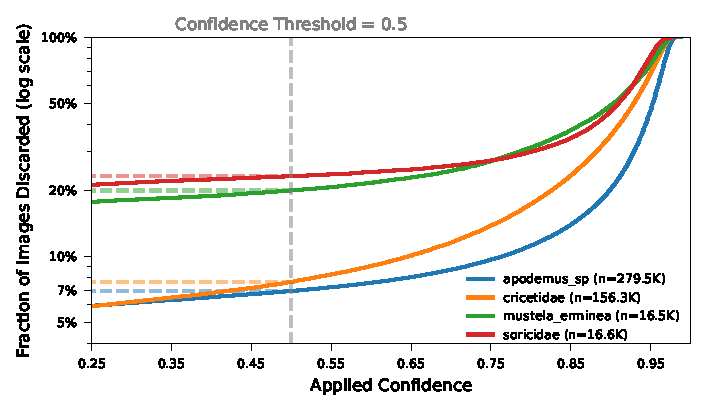
\includegraphics{figures/discarded_img_by_conf.pdf}
        \caption{Fraction of images discarded per category for a detection confidence threshold of 0.5.}
        \label{fig:lost_images}
        \end{figure}

        \begin{figure}[ht]
        \centering
        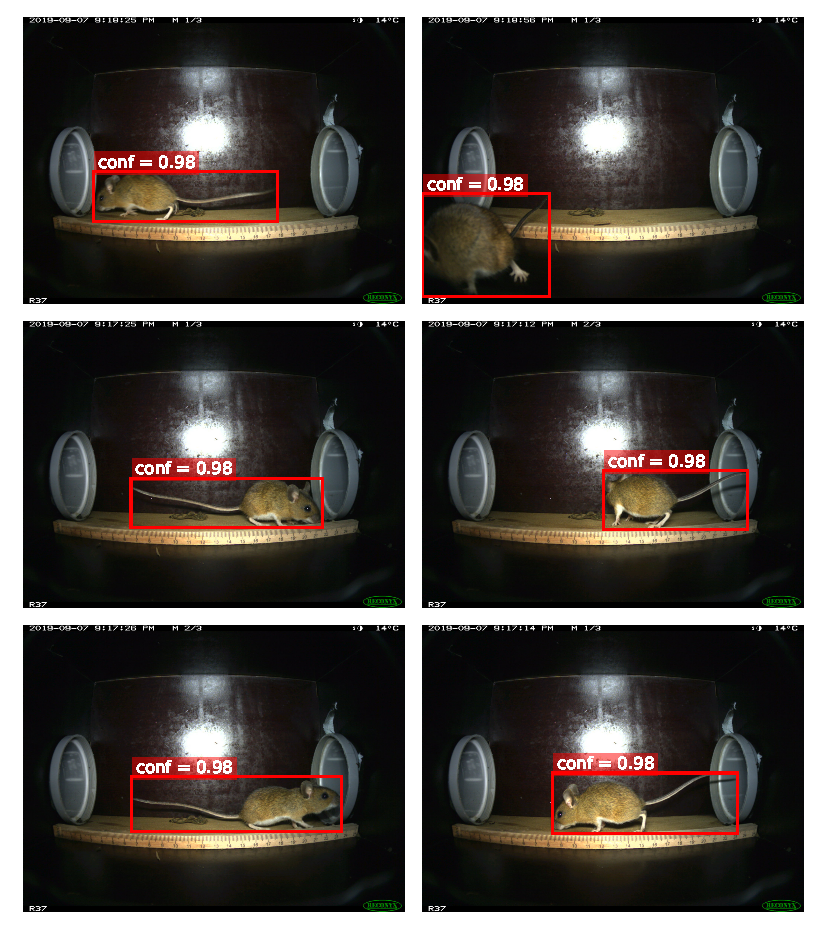
\includegraphics{figures/detections_on_a_sequence.pdf}
        \caption{Example of how the detections look like. The bounding boxes are the six highest confidence detections for the sequence 1001824 a sample from the \textit{apodemus\_sp} category.}
        \label{fig:detection_example}
        \end{figure}

        \subsubsection{Image Processing}
        To process the images a custom transformation pipline was implemented using transform version 2 from the torchvision library and a custom crop function.
        This transformation is applied on the fly by the PyTorch DataLoader.
        Cropping was done using the BBoxes from the MD detection extending the BBox in order to cut the ratio expected by the model applied.
        In the case that the extended BBox surpasses the image border the image is padded with black pixels.
        After cropping the image is resized to the expected input size of the model.
        The images are then converted to a tensor and normalized using the mean and standard deviation calculated on the dataset itself.
        To calculate mean and standard deviation the whole dataset was used since it is quite resource intensive to calculate and the same values are used for all folds.
        To create the most accurate mean and standard deviation for the actual model input only the best BBox area per image is used.
        Data augmentation a well established way to improve model's generalization \autocite{shortenSurveyImageData2019} was implemented and considered as an option but not actually used in the end.

        \subsubsection{Data Splitting}

        The dataset is split into five folds using a stratified split based on the classes.
        A custom helper function was implemented to ensure the splits are done on a sequence level, meaning no sequence is ever split between folds, while still maintaining a balanced distribution of images across the folds.
        For each class in the dataset, all the sequences are shuffled using a fixed seed for reproducibility resulting in two lists: one with the sequence ids and one with the corresponding sequence lengths.
        To build five stratified folds, it steps through the shuffled list of sequence-lengths and chooses cut-points so that each fold's sum of images is as close as possible to one-fifth of that class's total images.
        In this way, every fold ends up with roughly the same number of images per class, and no sequence is ever split between folds.

    \subsection{Model}

    In this project, a selection of models from the torchvision library was tested to classify the images. 
    Every model was both trained from scratch and fine-tuned using the weights of a model pre-trained on ImageNet \autocite{dengImageNetLargescaleHierarchical2009}.
    A custom helper function was implemented to adapt the last layer of the model to fit the number of classes in the dataset when the model is loaded.
    The models used in this project are:

    \begin{itemize}
        \item \textbf{EfficientNet-B0} \autocite{tanEfficientNetRethinkingModel2019}:  
        A Convolutional Neural Network architecture that uses a compound scaling method to uniformly scale network width, depth, and resolution.  
        The B0 variant is the baseline model from which larger EfficientNets are derived.  

        \item \textbf{DenseNet-169} \autocite{huangDenselyConnectedConvolutional2017}:  
        A densely connected convolutional network with 169 layers in which each layer receives feature-maps from all preceding layers, fostering feature reuse and improved gradient flow.  

        \item \textbf{ResNet-50} \autocite{heDeepResidualLearning2016}:  
        A 50‐layer Residual Network that introduces skip connections (residual blocks) to alleviate the vanishing-gradient problem, enabling training of very deep models.  

        \item \textbf{ViT-B\_16} \autocite{dosovitskiyImageWorth16x162021}:  
        The “Base” Vision Transformer model which splits an image into \(16\times 16\) patches, linearly embeds them, and processes the resulting sequence with a standard Transformer encoder.  
    \end{itemize}

    \subsection{Training}

    The training process is divided into four main steps repeated for each fold of the cross-validation:
    \begin{enumerate}
        \item Loading the dataset and applying the preprocessing steps described above.
        \item Initializing the model with the appropriate architecture and adapting the last layer to match the classes.
        \item Training the model for the current fold using the training set only keeping the last and the best version of the model.
        \item The best version of the model is loaded to predict the whole dataset for later evaluation.
    \end{enumerate}

    During training, the loss is calculated using the cross-entropy loss function with the class weights calculated on the current training set.
    To adjust the model parameters, the AdamW optimizer \autocite{loshchilovDecoupledWeightDecay2019} is used with a weight decay of $10^{-5}$ and an initial learning rate of $10^{-4}$.
    The learning rate is adjusted using a cosine annealing scheduler \autocite{loshchilovSGDRStochasticGradient2017} over 50 epochs.
    A maximum of 50 epochs where trained, but an early stopping callback was implemented monitoring the validation loss with a patience of 10 epochs.
    The logging is done using the tensorboard logger, which is integrated into PyTorch Lightning and an additional custom CSV logger for easier log access for evaluation.
    A batch size of 64 was used for training -- and doubled for validation and prediction.
    Predicting the whole dataset the predicted class for each sample and the confidence scores per class where saved to a CSV file for later evaluation

    \subsection{Sequence Classification}
    Since the data is grouped into sequences and the classification is done per image, an additional step is performed to classify the sequences.
    This step is only performed after the model has been trained and the predictions for the whole dataset are available.
    To classify the sequences, the image-level predictions are aggregated by sequence ID and the confidence scores for each class are summed across all images in the sequence.
    To normalize this summed confidences, they each are divided by the total sum of all summed confidences in that sequence.
    From this normalized confidences, the class with the highest confidence is selected as the predicted class for the sequence.

    \subsection{Evaluation}

    The evaluation is done using the predictions created by the best version of every model for each fold.
    Both the image-level and sequence-level predictions are evaluated using the balanced accuracy score \autocite{brodersenBalancedAccuracyIts2010} as the main metric.
    The balanced accuracy score is calculated using the following formula:
    \begin{equation}
    \text{Balanced Accuracy}
    \;=\;
    \frac{1}{K} \sum_{c=1}^{K}
        \frac{TP_{c}}{\,TP_{c} + FN_{c}\,}
    \end{equation}

    \noindent where:
    \begin{description}
    \item[$K$] is the total number of classes.
    \item[$TP_{c}$] (true positives for class $c$) is the count of samples whose true label is $c$ and whose predicted label is also $c$.
    \item[$FN_{c}$] (false negatives for class $c$) is the count of samples whose true label is $c$ but whose predicted label is not $c$.
    \end{description}


    \subsection{Hardware and Software}

    This project was processed on the IUNR HPC cluster using node 301, an HPE Apollo 6500 Gen10+ node running Rocky Linux 8. 
    The node is equipped with 8 NVIDIA L40S GPUs (48 GB each), dual AMD EPYC 7742 processors, 512 cores, and 5800 GB of storage, providing the computational power needed for high-performance tasks.

    The software environment was set up using micromamba, a lightweight version of conda, to manage the dependencies and packages required for the project.
    A \textit{environment.yml} file is provided in the GitHub repository to reproduce the environment.
    The Python version and used packages are as follows:

    \begin{itemize}
        \item Python 3.10.16
        \item NumPy 2.2.4
        \item pandas 2.2.3
        \item Matplotlib 3.10.1
        \item scikit-learn 1.6.1
        \item PyTorch 2.5.1
        \item PyTorch Lightning 2.5.1
        \item Pillow 9.4.0
    \end{itemize}


